\documentclass{standalone}
\usepackage{tikz}
\usetikzlibrary{patterns, positioning}


\begin{document}
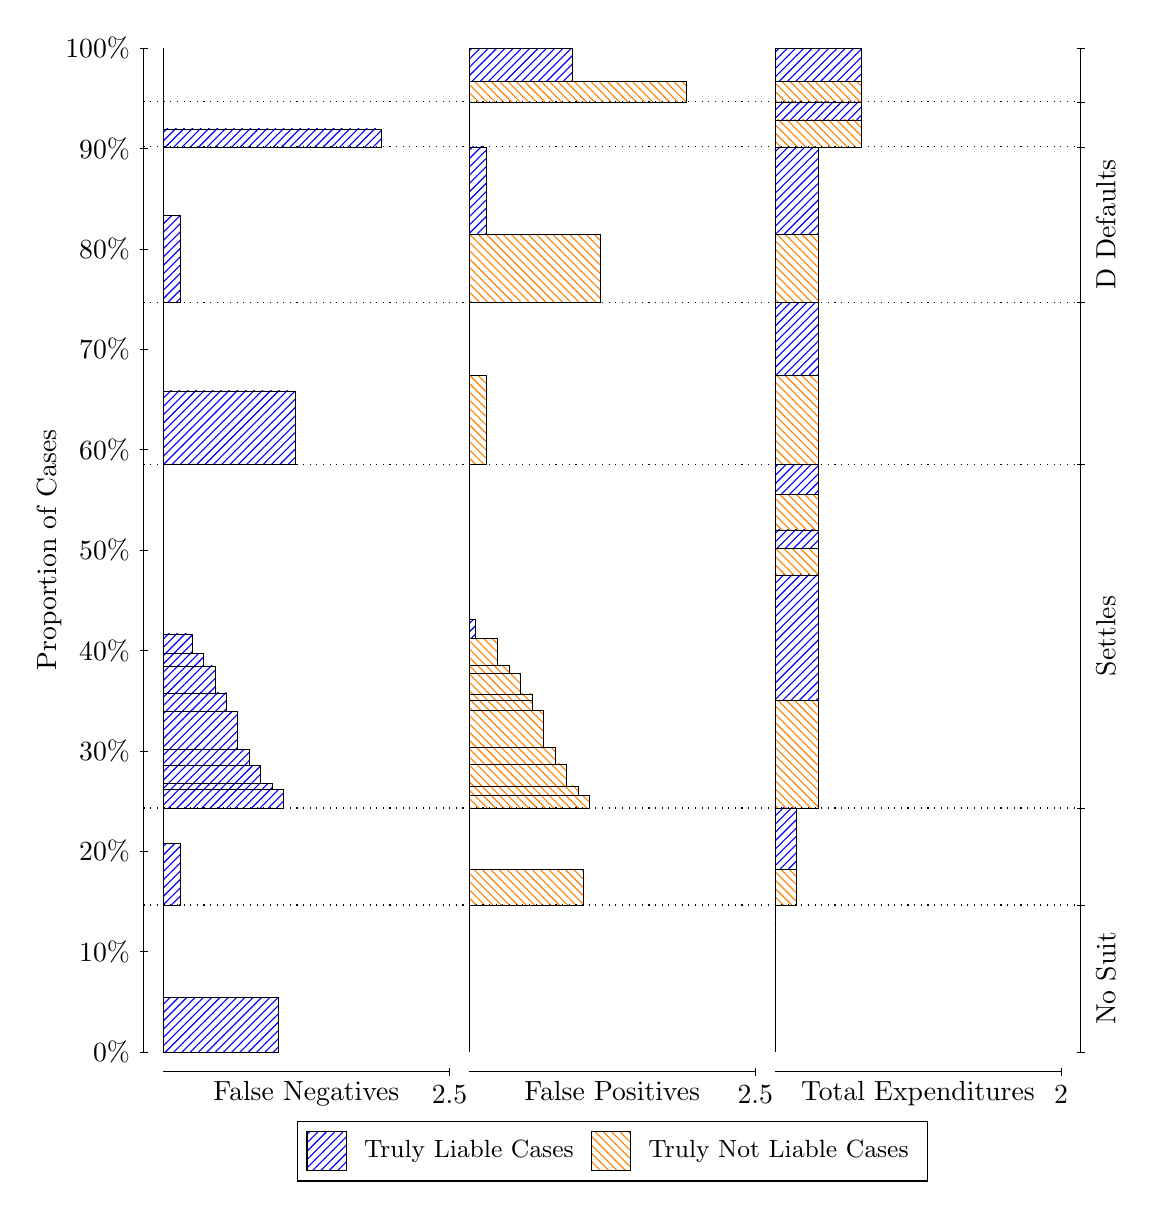
\begin{tikzpicture}
\draw[black, very thin] (1.5,1.75) -- (1.5,14.5);
\node[rotate=90, text=black, anchor=center] at (0.3, 8.125) {Proportion of Cases};
\draw[black, very thin] (1.45,1.75) -- (1.55,1.75);
\node[text=black, anchor=east] at (1.45, 1.75) {0\%};
\draw[black, very thin] (1.45,3.025) -- (1.55,3.025);
\node[text=black, anchor=east] at (1.45, 3.025) {10\%};
\draw[black, very thin] (1.45,4.3) -- (1.55,4.3);
\node[text=black, anchor=east] at (1.45, 4.3) {20\%};
\draw[black, very thin] (1.45,5.575) -- (1.55,5.575);
\node[text=black, anchor=east] at (1.45, 5.575) {30\%};
\draw[black, very thin] (1.45,6.85) -- (1.55,6.85);
\node[text=black, anchor=east] at (1.45, 6.85) {40\%};
\draw[black, very thin] (1.45,8.125) -- (1.55,8.125);
\node[text=black, anchor=east] at (1.45, 8.125) {50\%};
\draw[black, very thin] (1.45,9.4) -- (1.55,9.4);
\node[text=black, anchor=east] at (1.45, 9.4) {60\%};
\draw[black, very thin] (1.45,10.675) -- (1.55,10.675);
\node[text=black, anchor=east] at (1.45, 10.675) {70\%};
\draw[black, very thin] (1.45,11.95) -- (1.55,11.95);
\node[text=black, anchor=east] at (1.45, 11.95) {80\%};
\draw[black, very thin] (1.45,13.225) -- (1.55,13.225);
\node[text=black, anchor=east] at (1.45, 13.225) {90\%};
\draw[black, very thin] (1.45,14.5) -- (1.55,14.5);
\node[text=black, anchor=east] at (1.45, 14.5) {100\%};

\draw[black, very thin] (13.4,1.75) -- (13.4,14.5);
\draw[black, very thin] (13.35,1.75) -- (13.45,1.75);
\node[anchor=west] at (13.35, 1.75) {};
\draw[black, very thin] (13.35,3.6171) -- (13.45,3.6171);
\node[anchor=west] at (13.35, 3.6171) {};
\draw[black, very thin] (13.35,4.8485) -- (13.45,4.8485);
\node[anchor=west] at (13.35, 4.8485) {};
\draw[black, very thin] (13.35,9.2147) -- (13.45,9.2147);
\node[anchor=west] at (13.35, 9.2147) {};
\draw[black, very thin] (13.35,11.272) -- (13.45,11.272);
\node[anchor=west] at (13.35, 11.272) {};
\draw[black, very thin] (13.35,13.245) -- (13.45,13.245);
\node[anchor=west] at (13.35, 13.245) {};
\draw[black, very thin] (13.35,13.816) -- (13.45,13.816);
\node[anchor=west] at (13.35, 13.816) {};
\draw[black, very thin] (13.35,14.5) -- (13.45,14.5);
\node[anchor=west] at (13.35, 14.5) {};

\draw[black, very thin, pattern color=blue, pattern=north east lines] (1.75,1.75) rectangle (3.2033,2.4461);
\draw[black, very thin, pattern color=orange, pattern=north west lines] (1.75,2.4461) rectangle (1.75,3.6171);
\draw[black, very thin, pattern color=blue, pattern=north east lines] (1.75,3.6171) rectangle (1.968,4.3977);
\draw[black, very thin, pattern color=orange, pattern=north west lines] (1.75,4.3977) rectangle (1.75,4.8485);
\draw[black, very thin, pattern color=blue, pattern=north east lines] (1.75,4.8485) rectangle (3.276,5.0811);
\draw[black, very thin, pattern color=blue, pattern=north east lines] (1.75,5.0811) rectangle (3.1307,5.1634);
\draw[black, very thin, pattern color=blue, pattern=north east lines] (1.75,5.1634) rectangle (2.9853,5.3888);
\draw[black, very thin, pattern color=blue, pattern=north east lines] (1.75,5.3888) rectangle (2.84,5.5887);
\draw[black, very thin, pattern color=blue, pattern=north east lines] (1.75,5.5887) rectangle (2.6947,6.0735);
\draw[black, very thin, pattern color=blue, pattern=north east lines] (1.75,6.0735) rectangle (2.5493,6.3091);
\draw[black, very thin, pattern color=blue, pattern=north east lines] (1.75,6.3091) rectangle (2.404,6.6519);
\draw[black, very thin, pattern color=blue, pattern=north east lines] (1.75,6.6519) rectangle (2.2587,6.8146);
\draw[black, very thin, pattern color=blue, pattern=north east lines] (1.75,6.8146) rectangle (2.1133,7.0599);
\draw[black, very thin, pattern color=orange, pattern=north west lines] (1.75,7.0599) rectangle (1.75,9.2147);
\draw[black, very thin, pattern color=blue, pattern=north east lines] (1.75,9.2147) rectangle (3.4213,10.145);
\draw[black, very thin, pattern color=orange, pattern=north west lines] (1.75,10.145) rectangle (1.75,11.272);
\draw[black, very thin, pattern color=blue, pattern=north east lines] (1.75,11.272) rectangle (1.968,12.379);
\draw[black, very thin, pattern color=orange, pattern=north west lines] (1.75,12.379) rectangle (1.75,13.245);
\draw[black, very thin, pattern color=blue, pattern=north east lines] (1.75,13.245) rectangle (4.5113,13.474);
\draw[black, very thin, pattern color=orange, pattern=north west lines] (1.75,13.474) rectangle (1.75,13.816);
\draw[black, very thin, pattern color=orange, pattern=north west lines] (1.75,13.816) rectangle (1.75,14.08);
\draw[black, very thin, pattern color=blue, pattern=north east lines] (1.75,14.08) rectangle (1.75,14.5);
\draw[black, very thin, pattern color=orange, pattern=north west lines] (5.6333,1.75) rectangle (5.6333,2.921);
\draw[black, very thin, pattern color=blue, pattern=north east lines] (5.6333,2.921) rectangle (5.6333,3.6171);
\draw[black, very thin, pattern color=orange, pattern=north west lines] (5.6333,3.6171) rectangle (7.0867,4.0678);
\draw[black, very thin, pattern color=blue, pattern=north east lines] (5.6333,4.0678) rectangle (5.6333,4.8485);
\draw[black, very thin, pattern color=orange, pattern=north west lines] (5.6333,4.8485) rectangle (7.1593,5.0051);
\draw[black, very thin, pattern color=orange, pattern=north west lines] (5.6333,5.0051) rectangle (7.014,5.128);
\draw[black, very thin, pattern color=orange, pattern=north west lines] (5.6333,5.128) rectangle (6.8687,5.4074);
\draw[black, very thin, pattern color=orange, pattern=north west lines] (5.6333,5.4074) rectangle (6.7233,5.6193);
\draw[black, very thin, pattern color=orange, pattern=north west lines] (5.6333,5.6193) rectangle (6.578,6.0901);
\draw[black, very thin, pattern color=orange, pattern=north west lines] (5.6333,6.0901) rectangle (6.4327,6.2182);
\draw[black, very thin, pattern color=orange, pattern=north west lines] (5.6333,6.2182) rectangle (6.4327,6.2971);
\draw[black, very thin, pattern color=orange, pattern=north west lines] (5.6333,6.2971) rectangle (6.2873,6.556);
\draw[black, very thin, pattern color=orange, pattern=north west lines] (5.6333,6.556) rectangle (6.142,6.6645);
\draw[black, very thin, pattern color=orange, pattern=north west lines] (5.6333,6.6645) rectangle (5.9967,7.0033);
\draw[black, very thin, pattern color=blue, pattern=north east lines] (5.6333,7.0033) rectangle (5.706,7.2486);
\draw[black, very thin, pattern color=blue, pattern=north east lines] (5.6333,7.2486) rectangle (5.6333,9.2147);
\draw[black, very thin, pattern color=orange, pattern=north west lines] (5.6333,9.2147) rectangle (5.8513,10.341);
\draw[black, very thin, pattern color=blue, pattern=north east lines] (5.6333,10.341) rectangle (5.6333,11.272);
\draw[black, very thin, pattern color=orange, pattern=north west lines] (5.6333,11.272) rectangle (7.3047,12.138);
\draw[black, very thin, pattern color=blue, pattern=north east lines] (5.6333,12.138) rectangle (5.8513,13.245);
\draw[black, very thin, pattern color=orange, pattern=north west lines] (5.6333,13.245) rectangle (5.6333,13.587);
\draw[black, very thin, pattern color=blue, pattern=north east lines] (5.6333,13.587) rectangle (5.6333,13.816);
\draw[black, very thin, pattern color=orange, pattern=north west lines] (5.6333,13.816) rectangle (8.3947,14.08);
\draw[black, very thin, pattern color=blue, pattern=north east lines] (5.6333,14.08) rectangle (6.9413,14.5);
\draw[black, very thin, pattern color=orange, pattern=north west lines] (9.5167,1.75) rectangle (9.5167,2.921);
\draw[black, very thin, pattern color=blue, pattern=north east lines] (9.5167,2.921) rectangle (9.5167,3.6171);
\draw[black, very thin, pattern color=orange, pattern=north west lines] (9.5167,3.6171) rectangle (9.7892,4.0678);
\draw[black, very thin, pattern color=blue, pattern=north east lines] (9.5167,4.0678) rectangle (9.7892,4.8485);
\draw[black, very thin, pattern color=orange, pattern=north west lines] (9.5167,4.8485) rectangle (10.062,6.2182);
\draw[black, very thin, pattern color=blue, pattern=north east lines] (9.5167,6.2182) rectangle (10.062,7.8096);
\draw[black, very thin, pattern color=orange, pattern=north west lines] (9.5167,7.8096) rectangle (10.062,8.1484);
\draw[black, very thin, pattern color=blue, pattern=north east lines] (9.5167,8.1484) rectangle (10.062,8.381);
\draw[black, very thin, pattern color=orange, pattern=north west lines] (9.5167,8.381) rectangle (10.062,8.8273);
\draw[black, very thin, pattern color=blue, pattern=north east lines] (9.5167,8.8273) rectangle (10.062,9.2147);
\draw[black, very thin, pattern color=orange, pattern=north west lines] (9.5167,9.2147) rectangle (10.062,10.341);
\draw[black, very thin, pattern color=blue, pattern=north east lines] (9.5167,10.341) rectangle (10.062,11.272);
\draw[black, very thin, pattern color=orange, pattern=north west lines] (9.5167,11.272) rectangle (10.062,12.138);
\draw[black, very thin, pattern color=blue, pattern=north east lines] (9.5167,12.138) rectangle (10.062,13.245);
\draw[black, very thin, pattern color=orange, pattern=north west lines] (9.5167,13.245) rectangle (10.607,13.587);
\draw[black, very thin, pattern color=blue, pattern=north east lines] (9.5167,13.587) rectangle (10.607,13.816);
\draw[black, very thin, pattern color=orange, pattern=north west lines] (9.5167,13.816) rectangle (10.607,14.08);
\draw[black, very thin, pattern color=blue, pattern=north east lines] (9.5167,14.08) rectangle (10.607,14.5);
\draw[black, dotted] (1.5,3.6171) -- (13.4,3.6171);
\draw[black, dotted] (1.5,4.8485) -- (13.4,4.8485);
\draw[black, dotted] (1.5,9.2147) -- (13.4,9.2147);
\draw[black, dotted] (1.5,11.272) -- (13.4,11.272);
\draw[black, dotted] (1.5,13.245) -- (13.4,13.245);
\draw[black, dotted] (1.5,13.816) -- (13.4,13.816);
\draw[black, very thin] (1.75,1.5) -- (5.3833,1.5);
\node[text=black, anchor=north] at (3.5667, 1.5) {False Negatives};
\draw[black, very thin] (5.3833,1.45) -- (5.3833,1.55);
\node[text=black, anchor=north] at (5.3833, 1.45) {2.5};

\draw[black, very thin] (5.6333,1.5) -- (9.2667,1.5);
\node[text=black, anchor=north] at (7.45, 1.5) {False Positives};
\draw[black, very thin] (9.2667,1.45) -- (9.2667,1.55);
\node[text=black, anchor=north] at (9.2667, 1.45) {2.5};

\draw[black, very thin] (9.5167,1.5) -- (13.15,1.5);
\node[text=black, anchor=north] at (11.333, 1.5) {Total Expenditures};
\draw[black, very thin] (13.15,1.45) -- (13.15,1.55);
\node[text=black, anchor=north] at (13.15, 1.45) {2};

\node[text=black, centered, rotate=90] at (13.72, 2.6835) {No Suit};

\node[text=black, centered, rotate=90] at (13.72, 7.0316) {Settles};

\node[text=black, centered, rotate=90] at (13.72, 12.258) {D Defaults};



\draw (7.449999999999999,1.5) node[draw=none] (baseCoordinate) {};
\begin{scope}[align=center]
        \matrix[scale=0.5, draw=black, below=0.5cm of baseCoordinate, nodes={draw}, column sep=0.1cm]{
            \node[rectangle, draw, minimum width=0.5cm, minimum height=0.5cm, pattern color=blue, pattern=north east lines] {}; &
            \node[draw=none, font=\small, text=black] (B) {Truly Liable Cases}; &
            \node[rectangle, draw, minimum width=0.5cm, minimum height=0.5cm, pattern color=orange, pattern=north west lines] {}; &
            \node[draw=none, font=\small, text=black] (B) {Truly Not Liable Cases}; \\
            };
\end{scope}

\end{tikzpicture}
\end{document}